\chapter{Methodology}
\label{ch:methodology}

This chapter describes, in detail and in the order in which they are
executed, all the stages of the pipeline implemented for this thesis.
\Cref{sec:meth-formulation} formalizes the problem. \Cref{sec:meth-data}
describes the data sources. \Cref{sec:meth-filtering} explains how news
items are filtered and temporally aligned with market data.
\Cref{sec:meth-finbert} describes the FinBERT-based sentiment scoring
procedure. \Cref{sec:meth-aggregation} describes the sector-level
aggregation and smoothing of sentiment. \Cref{sec:meth-technical}
describes the technical indicators computed from S\&P 500 prices.
\Cref{sec:meth-dataset} describes the construction of the final
clustering dataset. \Cref{sec:meth-kmeans} describes the design of the
three \textit{K-Means} models (A, B and C). \Cref{sec:meth-hmm} describes
the Gaussian HMM used as a secondary comparison method.
\Cref{sec:meth-labeling} describes the regime-labeling methodology, and
\Cref{sec:meth-validation} describes the economic validation framework.

\section{Problem Formulation}
\label{sec:meth-formulation}

Let $t = 1, \dots, N$ index trading days. For each day $t$, a feature
vector $\mathbf{x}_t \in \mathbb{R}^d$ is constructed, composed of (a) a
set of \emph{technical} features derived from S\&P 500 OHLC prices, and
(b) a set of \emph{sentiment} features derived from financial news
headlines, aggregated at the sector level. The goal is to partition the
set $\{1, \dots, N\}$ into $K=3$ groups (clusters or states)
$\{C_0, C_1, C_2\}$ representing market regimes, such that the partition
is:

\begin{itemize}
  \item \textbf{statistically meaningful}, in the sense of producing
  internally cohesive and well-separated groups in feature space (assessed
  via the silhouette coefficient and PCA visualizations); and
  \item \textbf{economically meaningful}, in the sense that the
  subsequent returns of equity sectors differ systematically across
  groups (assessed via the sector-level economic validation framework of
  \Cref{sec:meth-validation}).
\end{itemize}

Three alternative definitions of $\mathbf{x}_t$ are considered (Models A,
B and C, \Cref{sec:meth-kmeans}), and two clustering algorithms are
applied to each definition: \textit{K-Means} (the primary method) and a
Gaussian Hidden Markov Model (the secondary, temporally-aware comparison
method, \Cref{sec:meth-hmm}).

\section{Data Sources}
\label{sec:meth-data}

\subsection{FNSPID Financial News Corpus}
\label{sec:meth-fnspid}

The sentiment signal is derived from the \textbf{FNSPID} (Financial News
and Stock Price Integration Dataset) corpus \cite{zhang2023fnspid}, which
contains time-stamped news headlines for US-listed companies. Each record
in the raw corpus consists, at minimum, of a publication timestamp, a
ticker symbol, and a headline (title) string.

\subsection{S\&P 500 Historical Constituents and OHLC Prices}
\label{sec:meth-sp500}

Daily OHLC (open-high-low-close) price data for the S\&P 500 index itself,
as well as for its individual constituents, is obtained via the
\texttt{yfinance} library. Because index membership has changed
substantially over the 2009--2024 period covered by this thesis (mergers,
delistings, additions and removals), a \textbf{historical constituents
table} is used to determine, for each date, which tickers were part of
the S\&P 500 at that time. This is essential to avoid
\emph{survivorship bias}: a naive approach that uses only the
\emph{current} (2024) list of S\&P 500 constituents to filter historical
news would systematically exclude news about companies that have since
been removed from the index (e.g., due to bankruptcy or acquisition),
biasing the resulting sentiment signal towards companies that have
historically performed well enough to remain in the index.

\subsection{GICS Sector Classification}
\label{sec:meth-gics}

Each ticker is mapped to one of the 11 \textbf{GICS} (Global Industry
Classification Standard) sectors using a mapping table
(\texttt{ticker\_gics\_mapping.csv}) built from Yahoo Finance sector
metadata. Because Yahoo Finance uses slightly different sector names than
the standard GICS taxonomy, a normalization step is applied (e.g.,
``Healthcare'' $\to$ \emph{Health Care}, ``Financials'' $\to$
\emph{Financial Services}, ``Consumer Cyclical'' $\to$ \emph{Consumer
Discretionary}, ``Consumer Defensive'' $\to$ \emph{Consumer Staples},
``Basic Materials'' $\to$ \emph{Materials}, ``Technology'' $\to$
\emph{Information Technology}). The resulting mapping covers 594 tickers
distributed across the 11 GICS sectors as shown in
\Cref{tab:gics-distribution}.

\begin{table}[H]
\centering
\caption{Distribution of S\&P 500 historical constituents across GICS sectors.}
\label{tab:gics-distribution}
\begin{tabular}{lr}
\toprule
\textbf{GICS Sector} & \textbf{Number of tickers} \\
\midrule
Industrials              & 94 \\
Financial Services       & 88 \\
Information Technology   & 76 \\
Consumer Discretionary   & 75 \\
Health Care              & 68 \\
Consumer Staples         & 39 \\
Real Estate              & 36 \\
Energy                   & 32 \\
Utilities                & 31 \\
Materials                & 30 \\
Communication Services   & 25 \\
\midrule
\textbf{Total}           & \textbf{594} \\
\bottomrule
\end{tabular}
\end{table}

\subsection{Storage Format: Parquet}
\label{sec:meth-parquet}

All intermediate and final datasets in the pipeline are stored using the
\textbf{Apache Parquet} columnar format rather than CSV. This choice is
motivated by three considerations specific to this project. First, the
FNSPID-derived sentiment tables involve millions of rows (one per
news--ticker--date triplet) with a mix of numeric (sentiment scores) and
categorical (sentiment labels) columns; Parquet's columnar layout and
built-in compression reduce both file size and load times by an order of
magnitude relative to CSV for this kind of data. Second, Parquet preserves
exact data types (e.g., \texttt{datetime64}, \texttt{float64}) across
read/write cycles, eliminating a common source of subtle bugs when
re-loading CSV files (such as dates being re-parsed as strings). Third,
because the pipeline involves multiple sequential stages
(filtering $\to$ sentiment scoring $\to$ aggregation $\to$ merging with
technical indicators $\to$ clustering), each of which reads the output of
the previous stage, the faster I/O provided by Parquet has a direct,
cumulative impact on iteration speed during development.

\section{News Filtering and Temporal Alignment}
\label{sec:meth-filtering}

Two filtering and alignment steps are applied to the raw FNSPID corpus
before sentiment scoring:

\begin{enumerate}
  \item \textbf{S\&P 500 membership filter.} A news item published on
  date $d$ for ticker $\tau$ is retained only if $\tau$ was a constituent
  of the S\&P 500 on date $d$, according to the historical constituents
  table described in \Cref{sec:meth-sp500}. This restricts the analysis to
  large-cap US equities and removes a substantial volume of news related
  to tickers that are not relevant to the S\&P 500-based regime detection
  problem addressed in this thesis.

  \item \textbf{Next-trading-day alignment.} Financial news is published
  continuously, including outside of market hours (evenings, weekends,
  holidays). To avoid \emph{look-ahead bias} --- i.e., using information
  in the sentiment signal for date $d$ that market participants could not
  yet have acted upon by the close of trading on date $d$ --- each news
  item is reassigned to the \emph{next open market day} on or after its
  publication date. Concretely, given the calendar of S\&P 500 trading
  days $\mathcal{T} = \{\tau_1 < \tau_2 < \dots\}$, a news item published
  on calendar date $d$ is assigned to
  $\tau^\star = \min\{\tau \in \mathcal{T} : \tau \ge d\}$. This guarantees
  that the sentiment computed for trading day $\tau^\star$ only reflects
  information that was publicly available no later than $\tau^\star$.
\end{enumerate}

\section{Sentiment Scoring with FinBERT}
\label{sec:meth-finbert}

Each filtered, date-aligned headline is scored using the
\texttt{ProsusAI/finbert} checkpoint, accessed through the Hugging Face
\texttt{transformers} \texttt{pipeline} API with the
\texttt{top\_k=None} option, which returns the full probability
distribution over the model's three output classes --- \emph{positive},
\emph{negative} and \emph{neutral} --- for each input headline.

\subsection{Preprocessing and Batching}

Headlines longer than 512 characters are truncated to the first 512
characters prior to tokenization, in line with FinBERT's maximum input
sequence length. To make inference tractable over a corpus spanning
millions of headlines, the model is run on GPU with a batch size of 64
headlines per forward pass. Batched GPU inference reduces the wall-clock
time of the sentiment-scoring stage from an impractical number of days
(at single-headline CPU throughput) to a few hours, which is what makes it
feasible to process more than a decade of FNSPID news for this thesis.

\subsection{Continuous Sentiment Score}

For each headline $i$, let $p_{\text{pos}}^{(i)}$, $p_{\text{neg}}^{(i)}$
and $p_{\text{neu}}^{(i)}$ denote the FinBERT output probabilities for the
\emph{positive}, \emph{negative} and \emph{neutral} classes, respectively
(with $p_{\text{pos}}^{(i)} + p_{\text{neg}}^{(i)} + p_{\text{neu}}^{(i)} =
1$). A continuous sentiment score is defined as:

\begin{equation}
  \label{eq:sentiment-score}
  s^{(i)} = p_{\text{pos}}^{(i)} - p_{\text{neg}}^{(i)} \in [-1, 1].
\end{equation}

This formulation has two useful properties. First, $s^{(i)} = 0$ both for
a headline classified as purely \emph{neutral} ($p_{\text{neu}}^{(i)}
\approx 1$) and for a headline for which the model is equally confident
about positive and negative sentiment ($p_{\text{pos}}^{(i)} \approx
p_{\text{neg}}^{(i)}$) --- both cases plausibly correspond to a headline
that conveys no net directional information. Second, $s^{(i)}$ is a
continuous quantity, which is more suitable for downstream aggregation
(averaging across many headlines per sector and day) than a discrete
class label would be.

\subsection{Categorical Sentiment Label and Tie-Breaking Rule}

In addition to the continuous score, a categorical sentiment label
$\ell^{(i)} \in \{\text{positive}, \text{negative}, \text{neutral}\}$ is
assigned using the arg-max rule:

\begin{equation}
  \label{eq:sentiment-label}
  \ell^{(i)} = \arg\max_{c \in \{\text{pos}, \text{neg}, \text{neu}\}}
  p_c^{(i)}.
\end{equation}

In the rare case of an exact tie between two or more classes, the
implementation resolves the tie by selecting the first class in the fixed
order (\emph{positive}, \emph{negative}, \emph{neutral}) returned by the
\texttt{transformers} pipeline, which in practice favors \emph{positive}
over \emph{negative}, and \emph{negative} over \emph{neutral}, in the
(extremely rare) event of exact numerical ties in the output
probabilities. Given that FinBERT's output probabilities are continuous
floating-point values, exact ties occur with negligible frequency and do
not materially affect the aggregated sector-level sentiment signal; the
categorical label is used primarily for descriptive/exploratory purposes,
while the continuous score $s^{(i)}$ from \Cref{eq:sentiment-score} is the
quantity actually propagated into the clustering dataset.

\section{Sector-Level Sentiment Aggregation and Smoothing}
\label{sec:meth-aggregation}

\subsection{Daily Aggregation by (Date, Sector)}

For each combination of trading day $\tau$ and GICS sector $g$, let
$\mathcal{I}_{\tau,g}$ denote the set of headlines assigned to day $\tau$
(via the next-trading-day alignment of \Cref{sec:meth-filtering}) whose
ticker belongs to sector $g$. Two daily statistics are computed:

\begin{equation}
  \label{eq:sector-mean}
  \overline{s}_{\tau,g} = \frac{1}{|\mathcal{I}_{\tau,g}|}
  \sum_{i \in \mathcal{I}_{\tau,g}} s^{(i)},
\end{equation}

\begin{equation}
  \label{eq:sector-std}
  \sigma_{\tau,g} = \sqrt{\frac{1}{|\mathcal{I}_{\tau,g}|}
  \sum_{i \in \mathcal{I}_{\tau,g}} \left(s^{(i)} - \overline{s}_{\tau,g}\right)^2}.
\end{equation}

The mean $\overline{s}_{\tau,g}$ (\texttt{sentiment\_avg\_<sector>})
captures the \emph{average tone} of news about sector $g$ on day $\tau$,
while the standard deviation $\sigma_{\tau,g}$
(\texttt{sentiment\_std\_<sector>}) captures the \emph{dispersion} or
\emph{disagreement} of sentiment across news items --- a day on which a
sector receives both very positive and very negative news (high
$\sigma_{\tau,g}$) is, intuitively, different from a day on which all news
about that sector point in the same direction (low $\sigma_{\tau,g}$),
even if the two days have a similar mean $\overline{s}_{\tau,g}$.

On days for which $|\mathcal{I}_{\tau,g}| \le 1$ (zero or one news item),
$\sigma_{\tau,g}$ is undefined (division by zero or by one with no
variance) and is therefore set to $0$ by convention, reflecting the
absence of disagreement when there is at most one data point. The wide
table of per-sector statistics is then constructed by pivoting the long
(date, sector, statistic) table into a wide table with one column per
(sector, statistic) combination. Any remaining missing values --- which
occur on days for which a given sector received \emph{no} news at all ---
are filled with $0$ for both the mean and the standard deviation columns,
under the interpretation that the absence of news corresponds to an
absence of sentiment signal (neutral, zero net tone) for that
sector on that day.

\subsection{Temporal Smoothing: Justification of the MA21 Window}
\label{sec:meth-smoothing}

The daily sector sentiment series $\overline{s}_{\tau,g}$ defined in
\Cref{eq:sector-mean} is, by construction, noisy: on any given day, a
sector's average sentiment can swing substantially depending on which
specific news items happened to be published, especially on
low-news-volume days. To obtain a signal that better reflects the
\emph{medium-term sentiment trend} of a sector --- which is arguably more
relevant for characterizing a market \emph{regime}, as opposed to a
single day's news flow --- a rolling moving average is applied:

\begin{equation}
  \label{eq:ma-smooth}
  \widetilde{s}_{\tau,g}^{(w)} = \frac{1}{w} \sum_{k=0}^{w-1}
  \overline{s}_{\tau-k,g}.
\end{equation}

To select the smoothing window $w$, an exploratory analysis was conducted
comparing $w \in \{5, 10, 21\}$ sessions (corresponding approximately to
one trading week, two trading weeks, and one trading month). For each
sector $g$ and window $w$, the standard deviation of the smoothed series
$\widetilde{s}_{\tau,g}^{(w)}$ was compared to the standard deviation of
the raw series $\overline{s}_{\tau,g}$, and the percentage \emph{noise
reduction} was computed as
$\left(1 - \mathrm{std}(\widetilde{s}^{(w)}) / \mathrm{std}(\overline{s})\right) \times 100\%$.
\Cref{tab:ma-noise-reduction} summarizes the results, averaged across the
11 GICS sectors.

\begin{table}[H]
\centering
\caption{Average noise reduction achieved by different moving-average smoothing windows applied to the daily sector sentiment series, averaged across the 11 GICS sectors.}
\label{tab:ma-noise-reduction}
\begin{tabular}{lccc}
\toprule
\textbf{Window} & \textbf{Mean noise reduction} & \textbf{Min} & \textbf{Max} \\
\midrule
MA5  & 47.4\% & 41.6\% & 51.7\% \\
MA10 & 58.4\% & 51.2\% & 64.1\% \\
MA21 & 66.5\% & 58.6\% & 72.6\% \\
\bottomrule
\end{tabular}
\end{table}

\Cref{fig:sentiment-smoothing} shows, for all 11 sectors, the raw and
MA21-smoothed sentiment series. \textbf{MA21 was selected} as the
smoothing window used to construct the \texttt{*\_smooth} sentiment
features used in Model C (\Cref{sec:meth-kmeans}), for two reasons. First,
it achieves the largest noise reduction among the three candidate windows
(66.5\% on average, compared to 47.4\% for MA5 and 58.4\% for MA10).
Second, a 21-session window corresponds to approximately one calendar
month of trading activity, which is a natural time scale for
\emph{regimes} as opposed to short-lived news cycles: a market regime that
persists for only a few days would be of limited practical use for the
risk-management and asset-allocation applications motivating this thesis
(\Cref{sec:motivation}). Windows longer than 21 sessions were not
explored, as they would begin to approach the typical persistence horizon
of the regimes themselves, risking over-smoothing the signal to the point
of removing the very transitions that the clustering models are intended
to detect.

\begin{figure}[H]
  \centering
  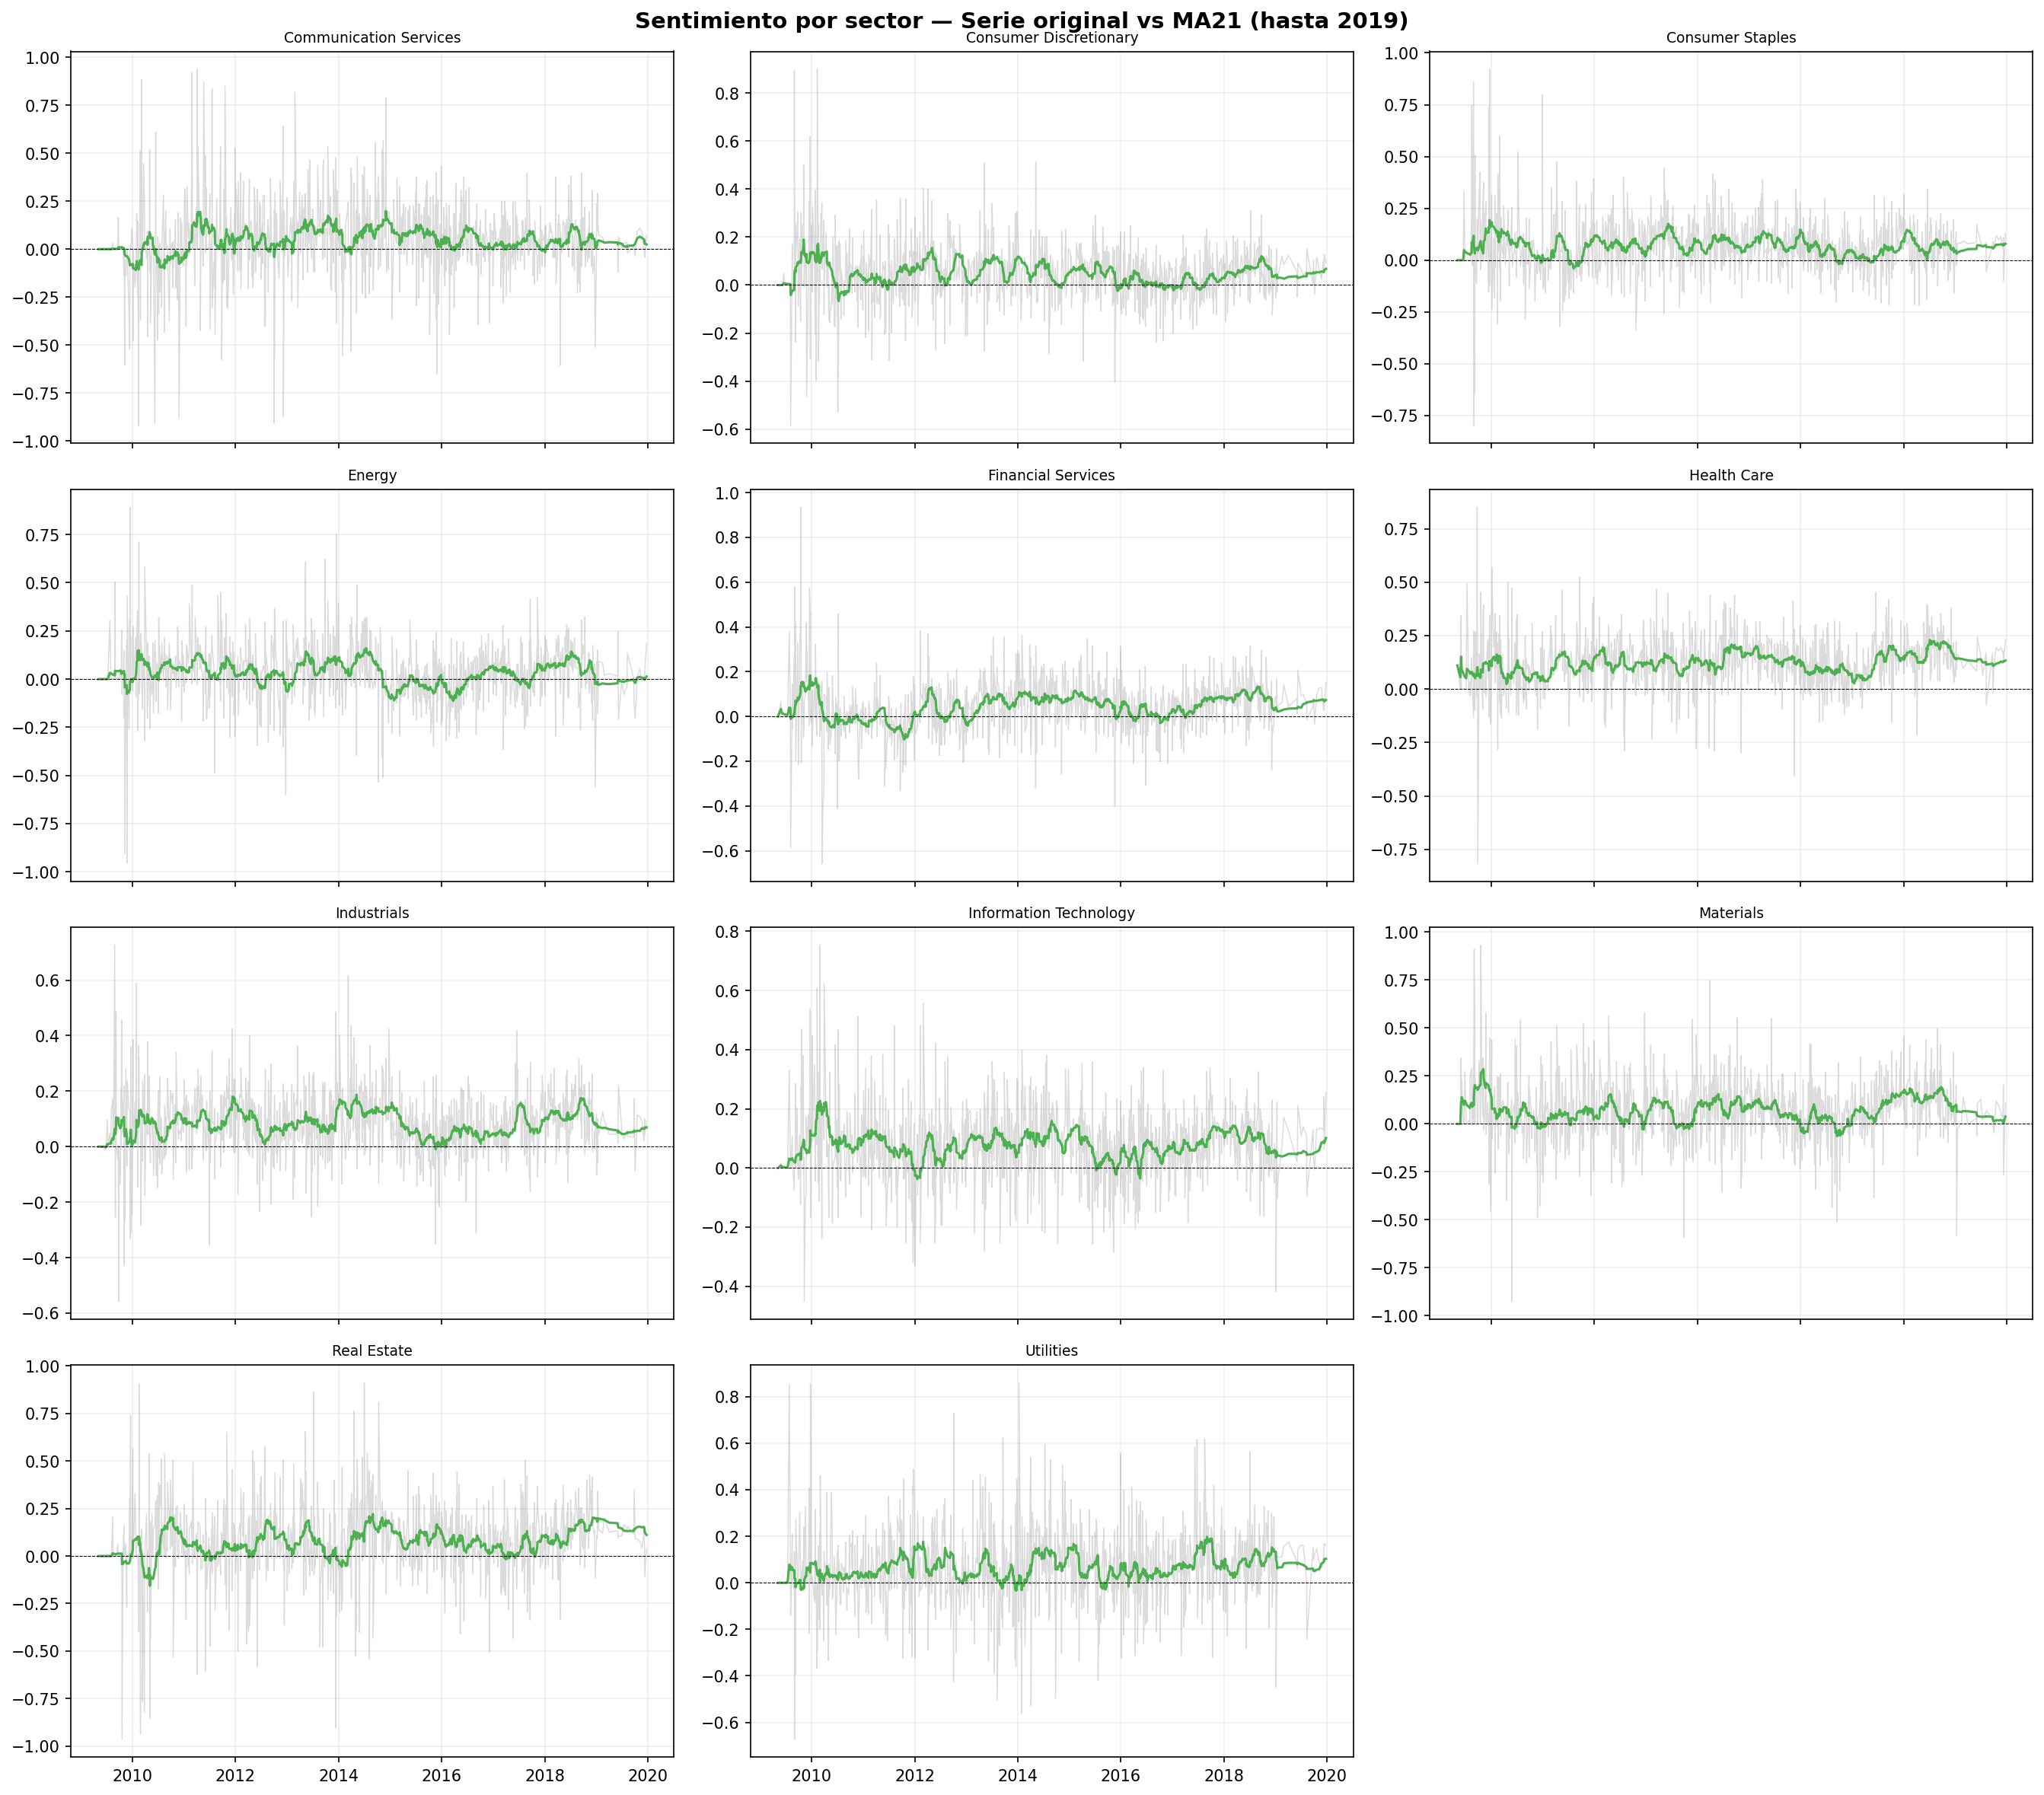
\includegraphics[width=0.95\textwidth]{figures/fig_sentiment_smoothing_summary.png}
  \caption{Raw (light) versus MA21-smoothed (dark) sector sentiment series for all 11 GICS sectors. The MA21 smoothing substantially reduces high-frequency noise while preserving medium-term sentiment trends.}
  \label{fig:sentiment-smoothing}
\end{figure}

It should be noted that this exploratory smoothing-window analysis was
conducted on an earlier development snapshot of the sentiment dataset
(covering 2009-05-08 to 2019-12-23, 1{,}073 daily observations); the final
clustering dataset used throughout the remainder of this thesis
(\Cref{sec:meth-dataset}) extends this range through February 2024. The
qualitative conclusion --- that MA21 offers the best trade-off between
noise reduction and preservation of medium-term trends --- is not
sensitive to this difference, since the smoothing window operates locally
on the time series and its relative noise-reduction properties depend on
the high-frequency statistical structure of the sentiment series rather
than on its total length.

\section{Technical Indicators}
\label{sec:meth-technical}

Nine technical indicators are computed from the daily closing price
$P_\tau$ of the S\&P 500 index. Let $r_\tau = \ln(P_\tau / P_{\tau-1})$
denote the daily log-return.

\begin{description}
  \item[Relative Strength Index (\texttt{RSI\_sp500}).] Computed using
  Wilder's exponential smoothing, implemented via an exponentially
  weighted moving average (EWM) with center-of-mass $\mathrm{com} =
  \mathrm{window} - 1 = 13$ (i.e., a 14-session RSI):
  \begin{equation}
    \label{eq:rsi}
    \mathrm{RSI}_\tau = 100 - \frac{100}{1 + RS_\tau}, \qquad
    RS_\tau = \frac{\mathrm{EWM}_{14}(\max(r_\tau, 0))}{\mathrm{EWM}_{14}(\max(-r_\tau, 0))}.
  \end{equation}

  \item[Moving-average ratios (\texttt{MA50\_ratio\_sp500},
  \texttt{MA200\_ratio\_sp500}).] The ratio of the current price to its
  50- and 200-session simple moving averages:
  \begin{equation}
    \label{eq:ma-ratio}
    \mathrm{MA}n\_\mathrm{ratio}_\tau = \frac{P_\tau}{\mathrm{SMA}_n(P)_\tau},
    \qquad n \in \{50, 200\}.
  \end{equation}
  Values above 1 indicate that the price is trading above its $n$-session
  average (an uptrend signal), and values below 1 indicate the opposite.

  \item[Momentum (\texttt{mom21\_sp500}, \texttt{mom126\_sp500}).] The
  percentage price change over the last 21 and 126 sessions
  (approximately one month and six months):
  \begin{equation}
    \label{eq:momentum}
    \mathrm{mom}n_\tau = \frac{P_\tau}{P_{\tau-n}} - 1, \qquad n \in \{21, 126\}.
  \end{equation}

  \item[Realized volatility (\texttt{vol30d\_sp500}, \texttt{vol252d\_sp500}).]
  The annualized standard deviation of log-returns over rolling windows of
  30 and 252 sessions (approximately one month and one year):
  \begin{equation}
    \label{eq:realized-vol}
    \mathrm{vol}n_\tau = \mathrm{std}\left(r_{\tau-n+1}, \dots, r_\tau\right)
    \times \sqrt{252}, \qquad n \in \{30, 252\}.
  \end{equation}

  \item[Return skewness (\texttt{skew30d\_sp500}, \texttt{skew252d\_sp500}).]
  The (Fisher-Pearson) sample skewness of log-returns over rolling windows
  of 30 and 252 sessions:
  \begin{equation}
    \label{eq:skewness}
    \mathrm{skew}n_\tau = \mathrm{skew}\left(r_{\tau-n+1}, \dots, r_\tau\right),
    \qquad n \in \{30, 252\}.
  \end{equation}
  Negative skewness indicates a distribution with a heavier left tail ---
  i.e., a higher relative likelihood of large negative returns --- which
  is a hallmark of crisis-type market dynamics.
\end{description}

These nine variables --- $\mathrm{RSI}$, two MA ratios, two momentum
measures, two realized volatilities, and two skewness measures --- form
the set \texttt{FEATURES\_TECH}, which is used directly in Model A and as
the technical component of Model B (\Cref{sec:meth-kmeans}).

\section{Clustering Dataset Construction}
\label{sec:meth-dataset}

The final clustering dataset is built by performing an \textbf{inner
merge}, on the \texttt{date} column, of (i) the wide table of sector-level
sentiment statistics (raw means and standard deviations, plus MA21-smoothed
means, for all 11 GICS sectors --- 33 sentiment columns in total) and (ii)
the table of nine technical indicators described in
\Cref{sec:meth-technical}. Technical-indicator column names are
standardized with a \texttt{\_sp500} suffix (e.g., \texttt{RSI} $\to$
\texttt{RSI\_sp500}, \texttt{mom126} $\to$ \texttt{mom126\_sp500},
\texttt{skew\_30d} $\to$ \texttt{skew30d\_sp500}) for consistency with the
sentiment column naming convention. Rows with missing values in any of
the nine technical features (which occur at the start of the series, where
the longest rolling windows --- 252 sessions --- are not yet fully
populated) are dropped.

The resulting dataset spans \textbf{2{,}009-05-08 to 2024-02-01} and
contains \textbf{1{,}132 daily observations} and \textbf{46 columns} in
total: 1 date column, 9 technical-indicator columns, 33 sentiment columns
(11 sectors $\times$ \{\texttt{avg}, \texttt{std}, \texttt{avg\_smooth}\}),
and (after clustering) the cluster-label columns described in the next
section.

\section{K-Means Clustering: Models A, B and C}
\label{sec:meth-kmeans}

\subsection{Selection of the Number of Clusters}

For each of the three feature configurations described below, the
\textit{K-Means} algorithm (\Cref{eq:soa-kmeans-objective}) is run for
$K \in \{2, \dots, 7\}$ with \texttt{k-means++} initialization, 10
independent initializations (\texttt{n\_init=10}) and
\texttt{random\_state=42} for reproducibility, after standardizing all
input features to zero mean and unit variance
(\texttt{StandardScaler}). For each $K$, the inertia (within-cluster sum
of squares, \Cref{eq:soa-kmeans-objective}) and the silhouette coefficient
(\Cref{eq:soa-silhouette}) are recorded. \Cref{fig:elbow-modelA,fig:elbow-modelB,fig:elbow-modelC}
show the resulting elbow/silhouette curves for Models A, B and C,
respectively. In all three cases, $K=3$ is selected: it lies at (or
immediately after) the ``elbow'' of the inertia curve, corresponds to a
local maximum or plateau of the silhouette curve, and --- crucially for
the interpretability goals of this thesis --- maps naturally onto the
\emph{Bull / Bear / Crisis} trichotomy discussed in
\Cref{sec:soa-kmeans}. A common value of $K=3$ across all three models
also ensures that Models A, B and C remain directly comparable.

\begin{figure}[H]
  \centering
  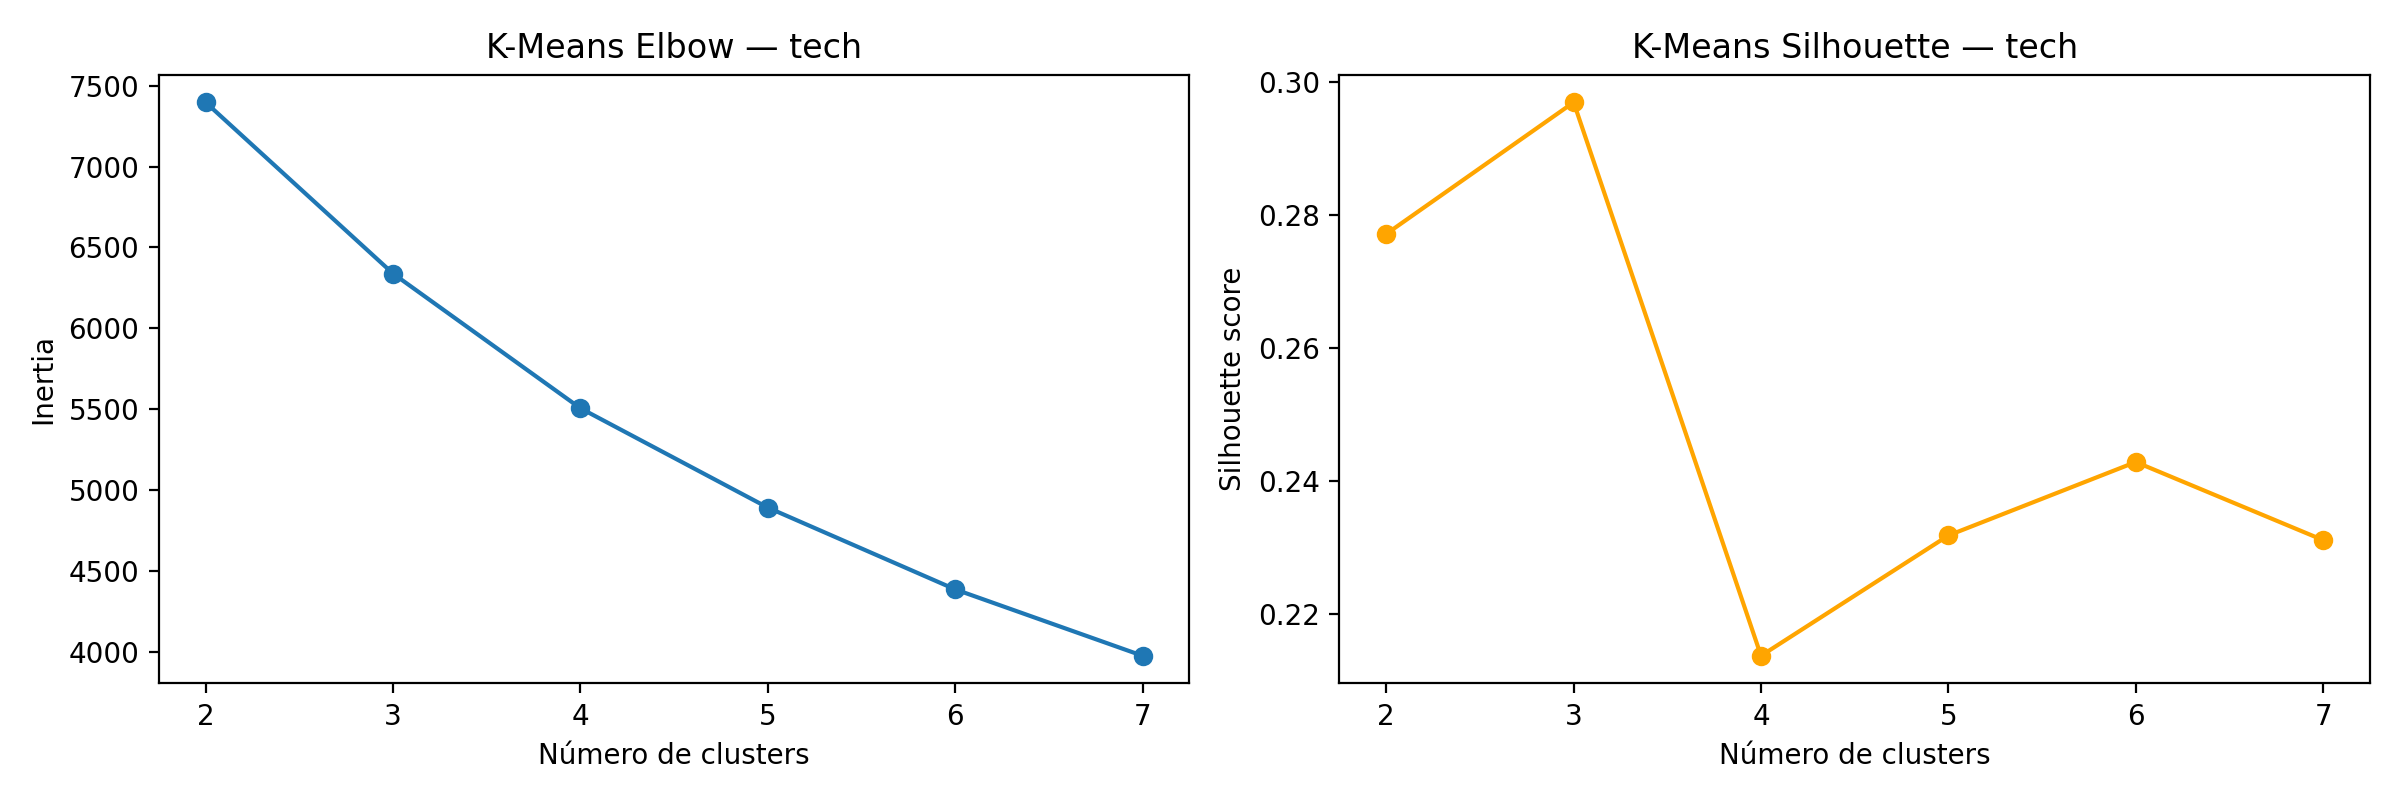
\includegraphics[width=0.95\textwidth]{figures/fig_elbow_modelA.png}
  \caption{Elbow (inertia) and silhouette curves for $K \in \{2,\dots,7\}$, Model A (technical indicators only).}
  \label{fig:elbow-modelA}
\end{figure}

\begin{figure}[H]
  \centering
  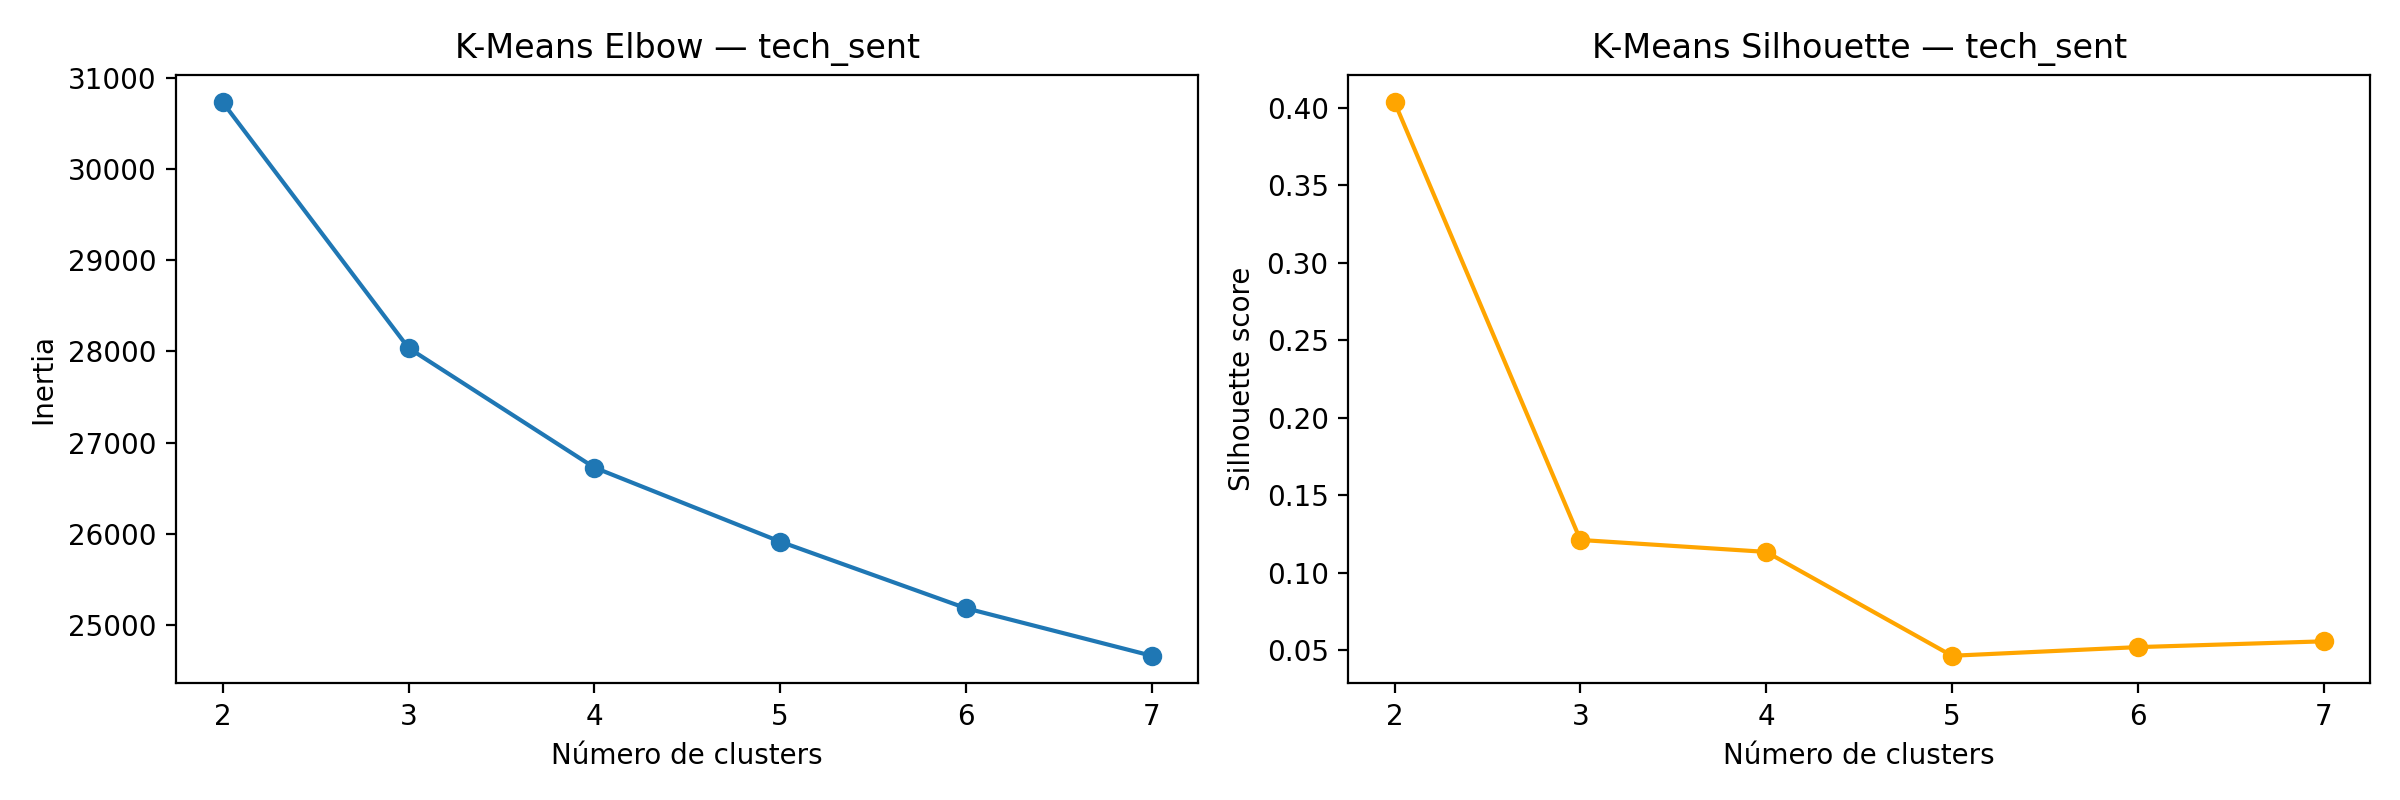
\includegraphics[width=0.95\textwidth]{figures/fig_elbow_modelB.png}
  \caption{Elbow (inertia) and silhouette curves for $K \in \{2,\dots,7\}$, Model B (technical indicators + raw sector sentiment).}
  \label{fig:elbow-modelB}
\end{figure}

\begin{figure}[H]
  \centering
  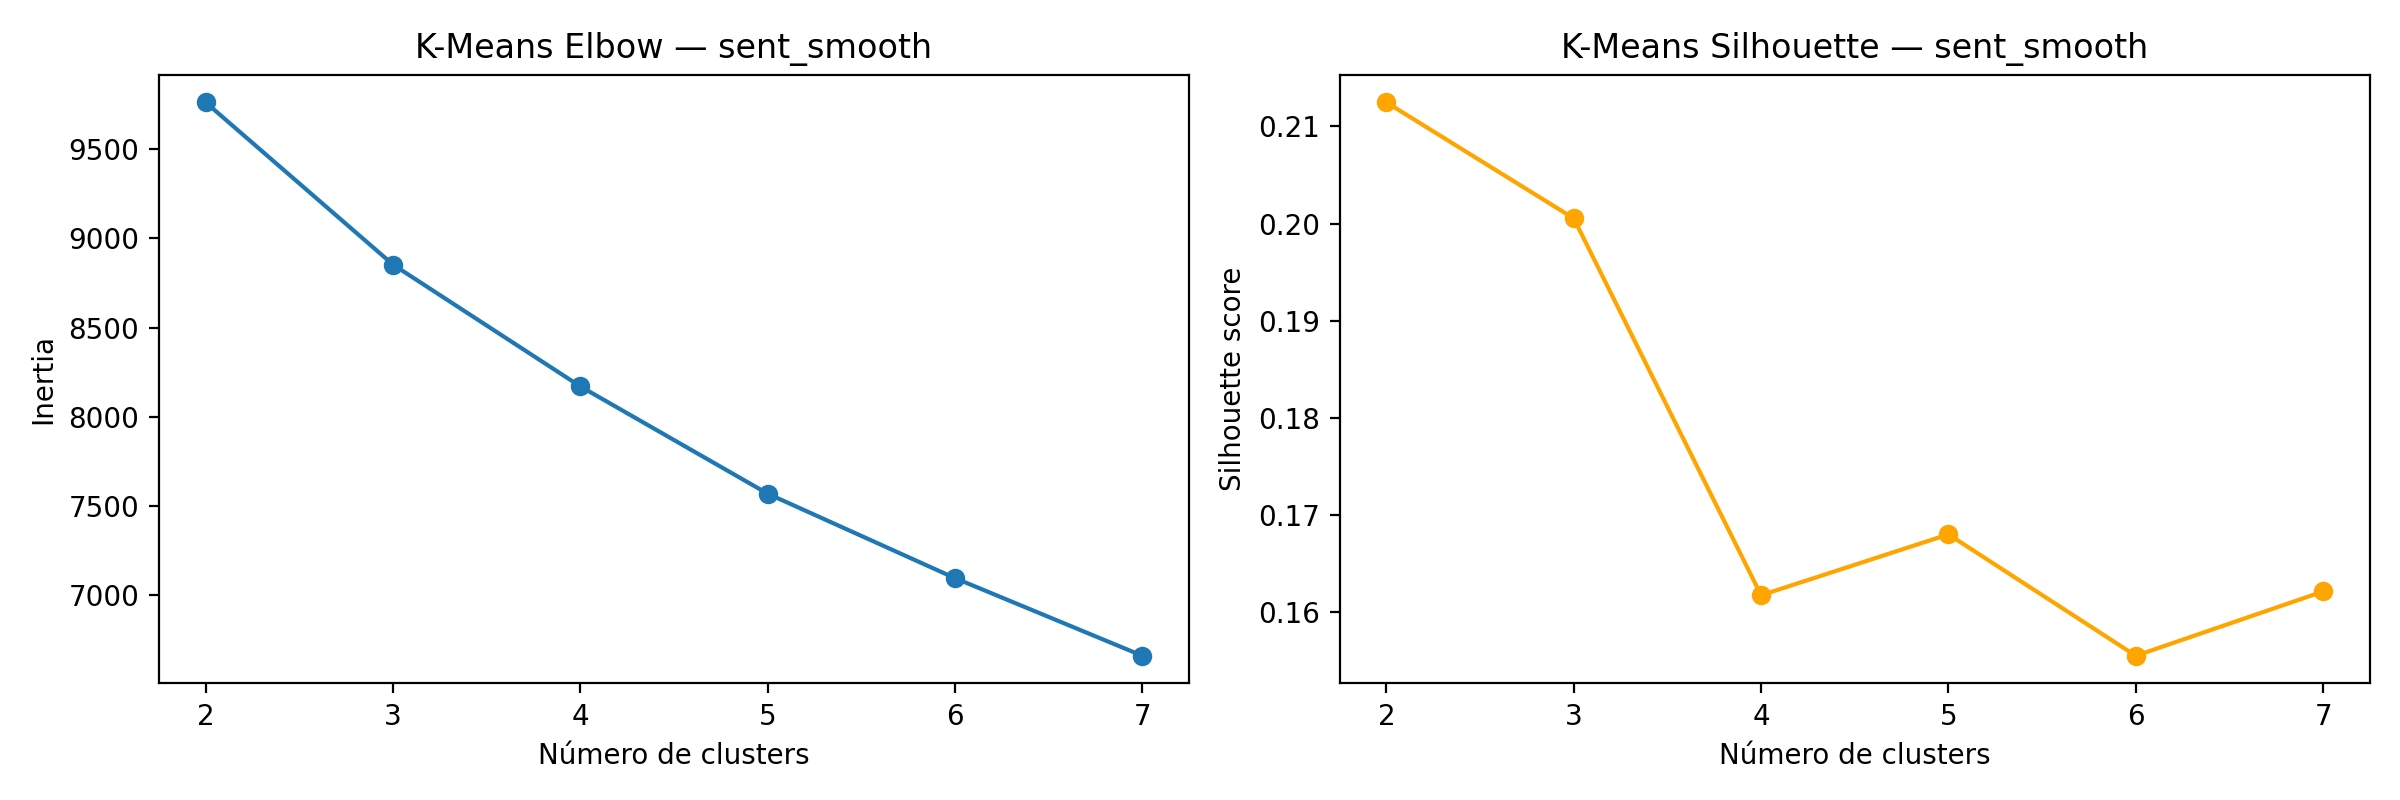
\includegraphics[width=0.95\textwidth]{figures/fig_elbow_modelC.png}
  \caption{Elbow (inertia) and silhouette curves for $K \in \{2,\dots,7\}$, Model C (smoothed sector sentiment only).}
  \label{fig:elbow-modelC}
\end{figure}

\subsection{Model A: Technical Indicators Only}

\textbf{Model A} uses exclusively the $d=9$ features in
\texttt{FEATURES\_TECH} (\Cref{sec:meth-technical}). This model serves as
the \emph{baseline}: it represents the ``classical'' approach to
clustering-based regime detection, using only price-derived information.
The resulting cluster labels are stored in the column
\texttt{kmeans\_tech}.

\subsection{Model B: Technical Indicators + Raw Sector Sentiment}

\textbf{Model B} augments the 9 technical features with the $22$ raw
(non-smoothed) sentiment columns --- \texttt{sentiment\_avg\_<sector>} and
\texttt{sentiment\_std\_<sector>} for each of the 11 GICS sectors --- for
a total of $d = 9 + 22 = 31$ features. This is the model that most
directly addresses the central research question of this thesis: does
adding contemporaneous sector-level sentiment information to the
technical baseline change the resulting regime partition, and if so, does
it do so in a way that is economically meaningful? The resulting cluster
labels are stored in the column \texttt{kmeans\_tech\_sent}.

\subsection{Model C: Smoothed Sector Sentiment Only}

\textbf{Model C} uses exclusively the $d=11$ MA21-smoothed sentiment means
(\texttt{sentiment\_avg\_<sector>\_smooth}, \Cref{sec:meth-smoothing}), with
no technical indicators at all. This model serves as a \emph{stress test}
of the sentiment signal in isolation: if sentiment alone were sufficient
to recover regimes with technical (price/volatility) characteristics
similar to those of Models A and B, this would suggest that sentiment is a
strong \emph{leading} indicator of the technical regime. Conversely, if
Model C's clusters show little technical differentiation, this indicates
that sentiment, while potentially informative as a complement
(cf.\ Model B), is not on its own a sufficient basis for regime detection.
The resulting cluster labels are stored in the column
\texttt{kmeans\_sent\_smooth}.

\Cref{tab:model-summary} summarizes the three models.

\begin{table}[H]
\centering
\caption{Summary of the three K-Means model configurations.}
\label{tab:model-summary}
\begin{tabular}{lllc}
\toprule
\textbf{Model} & \textbf{Feature set} & \textbf{Column} & \textbf{$d$} \\
\midrule
A & Technical indicators only & \texttt{kmeans\_tech} & 9 \\
B & Technical + raw sector sentiment (avg + std) & \texttt{kmeans\_tech\_sent} & 31 \\
C & Smoothed (MA21) sector sentiment only & \texttt{kmeans\_sent\_smooth} & 11 \\
\bottomrule
\end{tabular}
\end{table}

\section{Gaussian Hidden Markov Model: A Secondary Comparison Method}
\label{sec:meth-hmm}

To complement the \textit{K-Means} models with a method that explicitly
accounts for temporal transition dynamics
(\Cref{sec:soa-hmm}), a \textbf{Gaussian Hidden Markov Model} is fitted
using the \texttt{hmmlearn} implementation, with the following
configuration:

\begin{itemize}
  \item Number of hidden states: $K=3$ (matching the \textit{K-Means}
  models for comparability).
  \item Emission distributions: full covariance Gaussians
  (\texttt{covariance\_type="full"}), allowing each state to have its own
  unrestricted covariance structure across features.
  \item Optimization: Baum-Welch (EM) algorithm, \texttt{n\_iter=1000}
  maximum iterations.
  \item Numerical stability: a minimum covariance floor
  \texttt{min\_covar=1e-3} is imposed to avoid degenerate (near-singular)
  covariance estimates.
  \item Reproducibility: \texttt{random\_state=42}.
\end{itemize}

The HMM is fitted separately on the standardized feature sets
corresponding to \textbf{Model A} (the 9 technical features,
\texttt{hmm\_tech}) and \textbf{Model B} (the 31 technical + raw-sentiment
features, \texttt{hmm\_tech\_sent}), using the same
\texttt{StandardScaler}-transformed inputs as the corresponding
\textit{K-Means} model. After fitting, the most likely state sequence is
obtained via \texttt{hmm.predict()} (Viterbi decoding), yielding a state
label $h_\tau \in \{0,1,2\}$ for each trading day $\tau$.

Because $K$ is identical and the input feature sets are identical (after
standardization) to those of Models A and B, the HMM provides a
\emph{like-for-like} comparison point: any differences in the resulting
partitions (cluster sizes, temporal persistence, and --- most importantly
for this thesis --- economic differentiation across states, see
\Cref{ch:results}) can be attributed to the modeling choice (static
clustering vs. Markov-switching with explicit transition dynamics) rather
than to differences in the underlying data.

\section{Regime Labeling Methodology}
\label{sec:meth-labeling}

The raw cluster/state indices produced by \textit{K-Means} and the HMM
(integers $0,1,2$, with no inherent ordering or meaning) are mapped to the
economically meaningful labels \emph{Bull}, \emph{Bear} and
\emph{Crisis} by inspecting the \textbf{centroids} (cluster means) of the
nine technical features (\Cref{eq:rsi}--\Cref{eq:skewness}) for each
cluster. The labeling heuristic is as follows:

\begin{itemize}
  \item The cluster with \textbf{positive momentum} (\texttt{mom21},
  \texttt{mom126} $> 0$), \texttt{RSI} above 50, moving-average ratios
  above 1, and \emph{moderate} volatility is labeled \textbf{Bull}.
  \item The cluster with \textbf{negative (or near-zero) momentum},
  \texttt{RSI} below 50, moving-average ratios below or near 1, and
  elevated volatility is labeled \textbf{Bear}.
  \item The cluster with the \textbf{highest realized volatility}
  (particularly \texttt{vol252d}) and the most extreme (most negative)
  return skewness, often combined with a strong rebound in 126-session
  momentum, is labeled \textbf{Crisis}.
\end{itemize}

\Cref{tab:centroids-modelA} and \Cref{tab:centroids-modelB} report the
resulting centroids and cluster sizes for Models A and B (after applying
\texttt{StandardScaler} inversely, i.e., in the original units of each
feature), confirming that this heuristic assigns cluster index $0 \to$
Bull, $1 \to$ Bear and $2 \to$ Crisis consistently for both models.

\begin{table}[H]
\centering
\caption{Model A (technical-only): cluster centroids (mean feature values) and cluster sizes, $n=1{,}132$ observations.}
\label{tab:centroids-modelA}
\small
\begin{tabular}{lrrr}
\toprule
\textbf{Feature} & \textbf{Cluster 0 (Bull)} & \textbf{Cluster 1 (Bear)} & \textbf{Cluster 2 (Crisis)} \\
\midrule
RSI\_sp500          & 60.34 & 42.57 & 59.25 \\
MA50\_ratio\_sp500  & 1.0229 & 0.9739 & 1.0392 \\
MA200\_ratio\_sp500 & 1.0620 & 0.9877 & 1.1337 \\
mom21\_sp500        & 0.0227 & $-$0.0297 & 0.0281 \\
mom126\_sp500       & 0.0793 & $-$0.0075 & 0.2373 \\
vol30d\_sp500       & 0.1120 & 0.2005 & 0.1765 \\
vol252d\_sp500      & 0.1405 & 0.1670 & 0.3718 \\
skew30d\_sp500      & $-$0.1417 & $-$0.2704 & $-$0.4073 \\
skew252d\_sp500     & $-$0.3879 & $-$0.5259 & $-$0.2129 \\
\midrule
\textbf{$n$ (days)}  & \textbf{745} & \textbf{317} & \textbf{70} \\
\textbf{Share}       & 65.8\% & 28.0\% & 6.2\% \\
\bottomrule
\end{tabular}
\end{table}

\begin{table}[H]
\centering
\caption{Model B (technical + raw sentiment): cluster centroids (technical features only, for comparability with Model A) and cluster sizes, $n=1{,}132$ observations.}
\label{tab:centroids-modelB}
\small
\begin{tabular}{lrrr}
\toprule
\textbf{Feature} & \textbf{Cluster 0 (Bull)} & \textbf{Cluster 1 (Bear)} & \textbf{Cluster 2 (Crisis)} \\
\midrule
RSI\_sp500          & 60.50 & 43.34 & 60.11 \\
MA50\_ratio\_sp500  & 1.0235 & 0.9766 & 1.0374 \\
MA200\_ratio\_sp500 & 1.0647 & 0.9905 & 1.1190 \\
mom21\_sp500        & 0.0226 & $-$0.0265 & 0.0315 \\
mom126\_sp500       & 0.0841 & $-$0.0036 & 0.1997 \\
vol30d\_sp500       & 0.1110 & 0.1967 & 0.1734 \\
vol252d\_sp500      & 0.1417 & 0.1682 & 0.3438 \\
skew30d\_sp500      & $-$0.1430 & $-$0.2603 & $-$0.3975 \\
skew252d\_sp500     & $-$0.4137 & $-$0.4842 & $-$0.1016 \\
\midrule
\textbf{$n$ (days)}  & \textbf{720} & \textbf{342} & \textbf{70} \\
\textbf{Share}       & 63.6\% & 30.2\% & 6.2\% \\
\bottomrule
\end{tabular}
\end{table}

For \textbf{Model C}, the same $0 \to$ Bull, $1 \to$ Bear, $2 \to$ Crisis
mapping (based on the relative ordering of the smoothed-sentiment
centroids) is applied for consistency with Models A and B in the
economic-validation pipeline. However, as discussed in
\Cref{sec:results-modelC} of \Cref{ch:results}, when the \emph{technical}
feature centroids are computed for Model C's clusters (i.e., projecting
Model C's sentiment-only partition back onto the technical feature space),
the three clusters turn out to be \textbf{nearly indistinguishable} ---
e.g., \texttt{MA50\_ratio\_sp500} ranges only from $1.0086$ to $1.0134$
across Model C's three clusters, compared to a range of roughly $0.97$ to
$1.04$ for Models A and B. This observation is central to the discussion
of Model C as a methodologically informative negative result.

\section{Economic Validation Framework}
\label{sec:meth-validation}

The final stage of the methodology evaluates the \emph{economic} content
of the detected regimes, independently of the purely statistical
clustering metrics discussed in \Cref{ch:results}.

\subsection{Sector-Level Equally-Weighted Price Indices}

For each GICS sector $g$, an equally-weighted (EW) daily return series is
constructed from the historical S\&P 500 constituents belonging to sector
$g$ (\Cref{sec:meth-gics}). Daily close-to-close returns
$r_{\tau}^{(j)}$ are computed for every ticker $j$ in sector $g$ (using
\texttt{yfinance}-sourced, dividend- and split-adjusted closing prices,
cached locally as Parquet), and the sector return on day $\tau$ is defined
as the simple cross-sectional average:

\begin{equation}
  \label{eq:sector-return}
  R_{\tau,g} = \frac{1}{|\mathcal{J}_g|} \sum_{j \in \mathcal{J}_g} r_\tau^{(j)},
\end{equation}

where $\mathcal{J}_g$ is the set of tickers historically assigned to
sector $g$ that have available price data on day $\tau$.

\subsection{Regime Assignment to the Daily Price Calendar}

The cluster/state labels produced by Models A, B, C and the HMM are
defined on the 1{,}132-observation clustering dataset
(\Cref{sec:meth-dataset}), which does not necessarily cover every trading
day in the 2009--2024 sample with the same density as the daily price
calendar used for the sector return series. To align the two, the
cluster-label series is reindexed onto the full daily price calendar and
\textbf{forward-filled} (each day is assigned the most recently known
regime label), under the assumption that a detected regime remains in
effect until a new observation indicates otherwise. After reindexing, the
total number of (sector, regime)-labeled days is $3{,}695$ for every
model, distributed across the three regimes as shown in
\Cref{ch:results}.

\subsection{Economic Metrics}

For every combination of GICS sector $g$ and regime $\rho \in
\{\text{Bull}, \text{Bear}, \text{Crisis}\}$, let
$\{R_{\tau,g}\}_{\tau \in \mathcal{D}_{g,\rho}}$ denote the sector returns
on the subset of days $\mathcal{D}_{g,\rho}$ assigned to regime $\rho$,
with $n = |\mathcal{D}_{g,\rho}|$. The following metrics are computed
(combinations with $n < 10$ are excluded as statistically unreliable):

\begin{description}
  \item[Annualized return.] Computed from the total compounded return over
  the (non-contiguous) set of days assigned to the regime, annualized
  assuming $252$ trading days per year:
  \begin{equation}
    \label{eq:ann-return}
    \mu_{g,\rho} = \left(1 + \prod_{\tau \in \mathcal{D}_{g,\rho}}
    (1 + R_{\tau,g}) - 1\right)^{252/n} - 1.
  \end{equation}

  \item[Annualized volatility.]
  \begin{equation}
    \label{eq:ann-vol}
    \sigma_{g,\rho} = \mathrm{std}\left(\{R_{\tau,g}\}_{\tau \in
    \mathcal{D}_{g,\rho}}\right) \times \sqrt{252}.
  \end{equation}

  \item[Sharpe ratio.] With risk-free rate $r_f = 2\%$:
  \begin{equation}
    \label{eq:sharpe}
    \mathrm{Sharpe}_{g,\rho} = \frac{\mu_{g,\rho} - r_f}{\sigma_{g,\rho}}.
  \end{equation}

  \item[Maximum drawdown.] Computed on the cumulative return series
  $\mathrm{Cum}_\tau = \prod_{\tau' \le \tau, \tau' \in
  \mathcal{D}_{g,\rho}} (1 + R_{\tau',g})$ \emph{restricted to the days
  assigned to the regime} (i.e., treating the regime's days as if they
  were contiguous):
  \begin{equation}
    \label{eq:max-dd}
    \mathrm{MaxDD}_{g,\rho} = \min_\tau \frac{\mathrm{Cum}_\tau -
    \max_{\tau' \le \tau} \mathrm{Cum}_{\tau'}}{\max_{\tau' \le \tau}
    \mathrm{Cum}_{\tau'}}.
  \end{equation}
  Because the days in $\mathcal{D}_{g,\rho}$ are generally
  \emph{non-contiguous} in calendar time, $\mathrm{MaxDD}_{g,\rho}$ should
  be interpreted as a measure of the worst \emph{within-regime} compounded
  loss sequence, not as the drawdown of a literal buy-and-hold strategy.

  \item[Percentage of positive days.]
  $\mathrm{PctPos}_{g,\rho} = \frac{1}{n}\left|\{\tau \in
  \mathcal{D}_{g,\rho} : R_{\tau,g} > 0\}\right|$.

  \item[Best/worst single-day return.]
  $\mathrm{Best}_{g,\rho} = \max_{\tau \in \mathcal{D}_{g,\rho}} R_{\tau,g}$
  and $\mathrm{Worst}_{g,\rho} = \min_{\tau \in \mathcal{D}_{g,\rho}}
  R_{\tau,g}$. These extreme-value statistics are particularly informative
  for the \emph{Crisis} regime, where they capture the magnitude of the
  largest single-day moves (in either direction) that the regime is
  associated with.
\end{description}

For each metric, a heatmap with GICS sectors on the rows and regimes
(\emph{Bull}, \emph{Bear}, \emph{Crisis}) on the columns is generated,
providing a compact visual summary of how each regime manifests
economically across all 11 sectors simultaneously. These heatmaps, for
Models A, B and C, are presented and discussed in \Cref{ch:results}, with
the complete numerical tables reproduced in Annex~B.
